\chapter{Method}

 % Setup
 % - renvoyer au document de l'ensemble des choses que j'auraient aimés savoir dés le début


%  [résumer la situation et dire ce qu'il se passe dans ce chapitre. Raconter une histoire.]

Our exploration of the MEG data for the paradigm follows the classical steps of a MEG study:

\begin{itemize}
    \item Pre-Processing of the data. Our study started with the verification and cleaning of the data.
    \item Analysis in the sensor space. In this step we visualized the Evoked response of the different conditions. In order to find out when and how often the information is stored at the time of retrieval, we implemented a new procedure, based on Common Spatial Patterns (CSP). After determining the most salient time and frequency, we check the statistical significance of the response using cluster permutation tests.
          % \item [report visualization. CSP to see the patterns and see the frequencies and moments. Why at the beginning not at the end. We should have separated between the different length of sequence ??? Visualization of filters and paterns. Difficulties with the patterns. Should have taken just the first pattern].
    \item Source analysis. After having determined the frequency and the moment of maximum activation of the Working memory, we visualize the 3D response.
\end{itemize}

In order to pre-process the data, and to analyze the data in the sensor and source space, I based myself on the \href{https://github.com/mne-tools/mne-bids-pipeline}{MNE-BIDS-Pipeline}, which is still under development. As I wanted to use it for the time in working memory paradigm, I had to help implement the missing features I needed. The list of features to which I contributed is presented in the table \ref{Tab:PR}.

This chapter aims to detail the list of algorithms I implemented or improved in the pipeline to analyze our MEG data.

\begin{table}[ht]
    \centering
    \begin{tabular}{@{}| p{3cm}|p{9cm}| @{}}
        \hline
        Type             & Title                                                                                                                                                                                                                                                                       \\
        \hline
        New feature      & Add possibility to exclude runs from the analysis via the new exclude run setting.                                                                                                                                                                                          \\
        Code health      & Files docstrings in the preprocessing steps were updated.                                                                                                                                                                                                                   \\
        Behavior changes & Warn if using ICA and no EOG- or ECG-related ICs were detected.                                                                                                                                                                                                             \\
        New feature      & Added the possibility to have different runs for different subjects.                                                                                                                                                                                                        \\
        Behavior changes & Check that the baseline interval falls into the epoch interval.                                                                                                                                                                                                             \\
        Behavior changes & ica\_reject now also applies to ECG and EOG epochs.                                                                                                                                                                                                                         \\
        Bug fix          & The sanity check comparing the rank of the experimental data and the rank of the empty-room after Maxwell-filtering did not use the maxfiltered data.                                                                                                                       \\
        Bug fix          & epochs\_tmin and epochs\_tmax were named incorrectly in some test config files.                                                                                                                                                                                             \\
        Bug fix          & We now reject bad epochs by using ica\_reject before producing the "overlay" plots that show the evoked data before and after ICA cleaning in the `proc-ica\_report`.                                                                                                       \\
        New feature      & It is now possible to analyze the contrast using the Common Spatial Patterns in the time-frequency domain using the new script: 03b-time\_frequency\_csp.py. We also test the significance of the contrast between the two conditions using cluster permutation statistics. \\
        \hline
    \end{tabular}

    \caption[List of my contributions to the MNE-BIDS-Pipeline.]%
    {List of my contributions to the MNE-BIDS-Pipeline on \href{https://raw.githubusercontent.com/mne-tools/MNE-BIDS-Pipeline/main/docs/source/changes.md}{GitHub}.}
    \label{Tab:PR}
\end{table}

\section{Preprocessing of the data}

Before this internship, I had already worked on EEG data for the "Dream, sleep apnea" challenge and for the \href{https://github.com/crsegerie/bci_competition}{Inria - Brain Computer Interface Kaggle Challenge}. But on these two occasions, the data I had manipulated had already been cleaned by the competition organizers. This internship allowed me to realize the complexity of preprocessing data in brain imaging.

\subsection{The different steps of the preprocessing}

The different phases of the data preprocessing are as follows:

\begin{itemize}
    \item Finding bad channels: some channels of MEG recordings may be noisy or flat. They need to be identified and marked as bad so they are not taking into account during the analysis.
    \item Applying Maxwell filter: help to remove part of the sensors noise.
    \item Frequency filter: to remove non desired frequency bands.
    \item Creating epochs: epochs are data structures to represent equal-duration chuncks of MEG signals. When the recording session includes stimuli, epochs are often defined from 0.2 seconds before the stimulus to 0.5 seconds after. Otherwise, like in rest session, epochs are fixed and overlapping frames of the MEG signal.
    \item Computing evoked data: they are created by averaging MEG signal over several epochs. It is useful to study stimulus-evoked brain activity.
\end{itemize}


The figure \ref{cheat_sheet} summarizes the preprocessing step in the pipeline. At the beginning of my internship, I created this table in order to familiarize myself with the different scripts of the pipeline. Then, I added the main problems that occur in practice associated with each step as well as the main ideas of sanity checks to be performed after the execution of the pipeline.

\begin{figure}[ht]
    \centering
    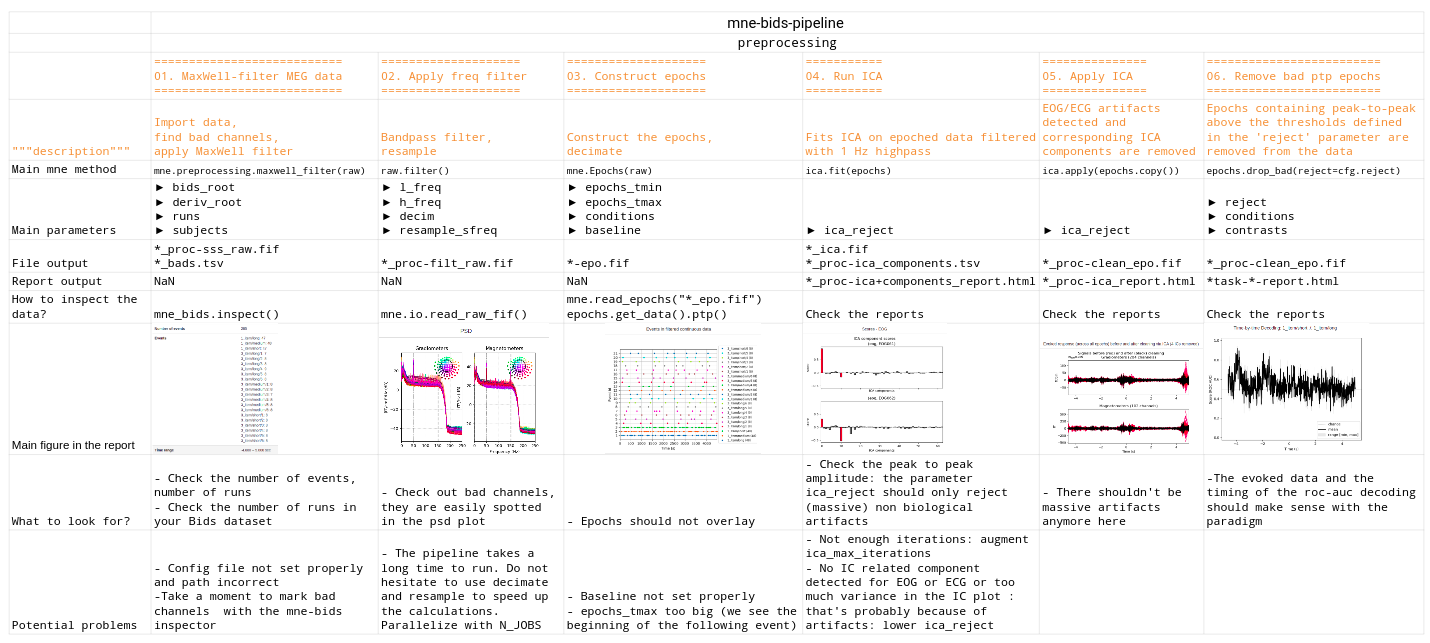
\includegraphics[width=15cm]{images_report/preprocessing/cheatsheet preprocessing.png}
    \caption[Summary of the preprocessing of the pipeline.]%
    {Summary of the preprocessing of the pipeline.}
    \label{cheat_sheet}
\end{figure}

\subsection{Highlight on the managment of artifacts}
\label{preprocessing_of_artifacts}


\begin{figure}[ht]
    \centering
    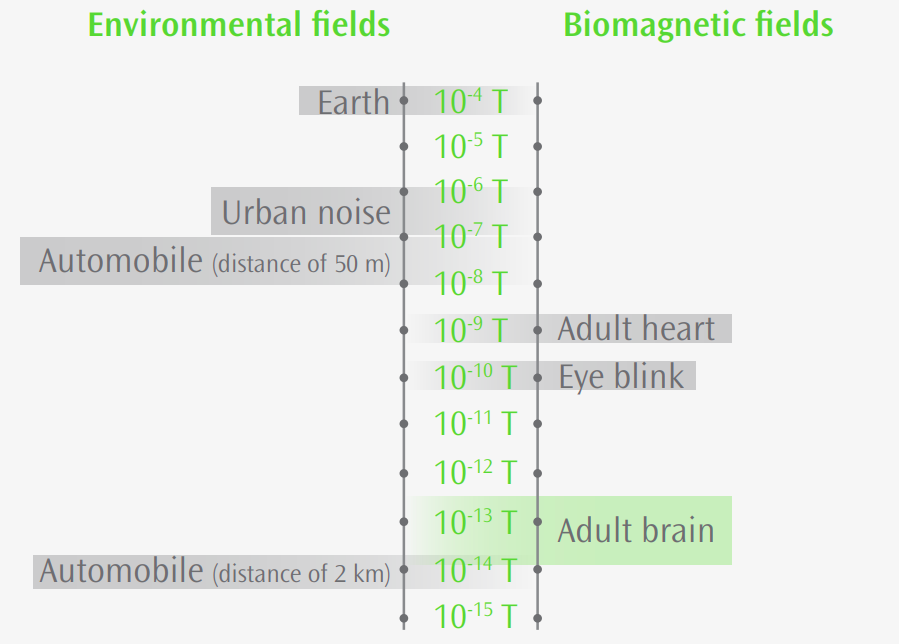
\includegraphics[width=7cm]{images_report/sensor/noise_order_of_magnitude.png}
    \caption[Scale of magnitude of different magnetic fields]%
    {Scale of magnitude of different magnetic fields}
    \label{noise_order_of_magnitude}
\end{figure}


An important point during the preprocessing is the order in which the data is rejected. Indeed, a major difficulty with raw data coming from cortical signals is the fact that these signals are extremely small. Although the data is recorded in a shielded chamber, the slightest noise can totally overwhelm the signal. Figure \ref{noise_order_of_magnitude} shows the scale of orders of magnitude, which makes it clear that the external noise is of an order of magnitude immeasurably larger than the neurological signals of interest.

Even after removing all the noise from the external environment, some of the so-called biological artifacts, such as heartbeats and blinks, must be removed by either discarding the contaminated time interval or separating the sources by using independent component analysis (ICA), which separates the heartbeat and blink sources from the rest of the signal.

The figure \ref{rejection_pipeline} allows to visualize the pipeline rejection of the MNE-BIDS-Pipeline.

\begin{figure}[ht]
    \centering
    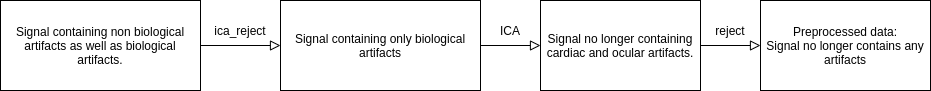
\includegraphics[width=15cm]{images_report/preprocessing/rejection_pipeline.png}
    \caption[Simplification of the BIDS-Pipeline rejection process.]%
    {Flow of the BIDS-Pipeline rejection process.}
    \label{rejection_pipeline}
\end{figure}

Here are the details of the procedure:
\begin{itemize}
    \item At the beginning the signal contains both biological artifacts (eye blink, heartbeat), and non biological artifacts. The latter are of an order of magnitude larger than the biological artifacts.
    \item We can start by filtering the different epochs using rejecting the epochs whose peak-to-peak amplitude exceeds the amplitude specified by the "ica\_reject" parameter. This parameter allows to filter signals that are 50 times larger than the nominal amplitude and therefore allows to make a first screening.
    \item The resulting signal does not contain any more redhibitory non-biological artifact, which allows to improve the convergence of the ICA (Independant Component Analysis), allowing to separate the sources for the ocular and cardiac artifacts.
    \item The ICA source separation does not work perfectly, so an additional step is required to reject the last artifacts using the "reject" parameter, which allows to filter the signals with a peak-to-peak amplitude 10 times higher than the nominal amplitude. The result is the preprocessed signal.
\end{itemize}

Even if the global pipeline rejection method was already established before my arrival, the experimental data revealed problems in the order of the filtering operations, and we thus improved a lot the automatic data preprocessing especially for difficult data that contains simulaneously biological and non-biological artifacts such as phase inversion fields. Figure \ref{fig:PR_ica} shows an example of ICA enhancement before and after our pull request that changes the order of operations, in particular by filtering out non-biological signals before the ICA.


\begin{figure}
    \centering
    \begin{subfigure}{.5\textwidth}
        \centering
        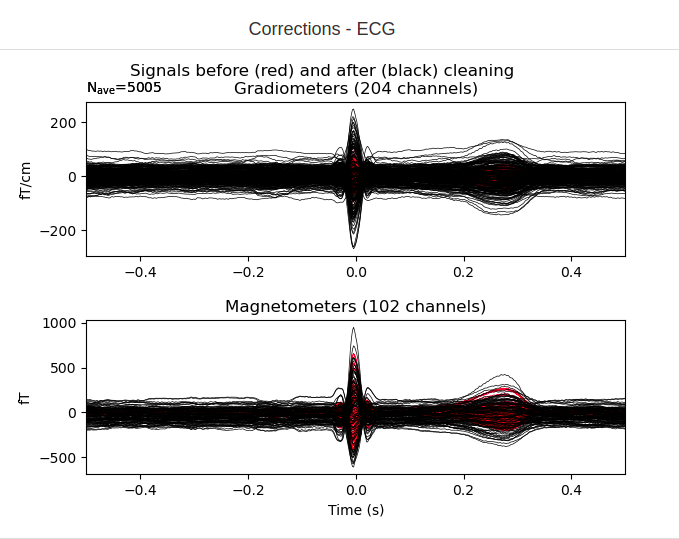
\includegraphics[width=1.\linewidth]{images_report/preprocessing/ica/ECG_ICA_before_PR.png}
        \caption{ICA correction before amelioration}
        \label{fig:before_ica_PR}
    \end{subfigure}%
    \begin{subfigure}{.5\textwidth}
        \centering
        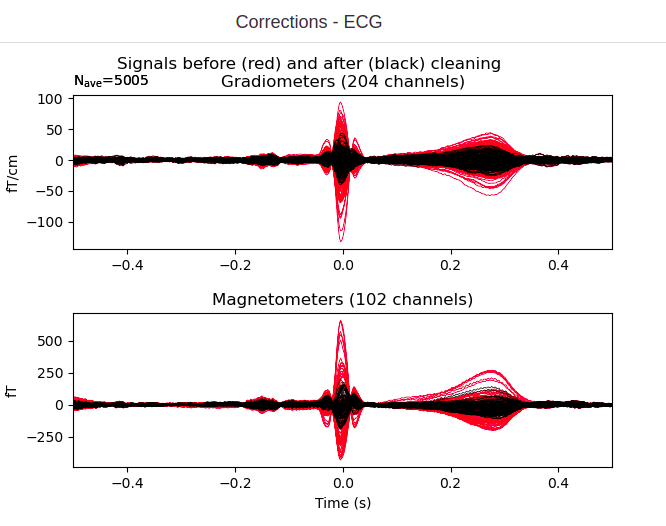
\includegraphics[width=1.\linewidth]{images_report/preprocessing/ica/ECG_ICA_after_PR.png}
        \caption{ICA correction after amelioration}
        \label{fig:after_ica_PR}
    \end{subfigure}
    \caption{We can see that after our pull request, the ICA is capable of reducing almost by 4 the peak to peak amplitude of the ECG artifact.}
    \label{fig:PR_ica}
\end{figure}



% [put an example of a heart or EOG ? Example of preprocessing reports.].

\section{Sensor Space: Finding the main time-frequency cluster}

[rappeller le source space]

\subsection{Insufficiency of the pipeline to analyze in a relevant way the MEG}

\begin{figure}[htb]
    \centering % <-- added
    \begin{subfigure}{0.25\textwidth}
        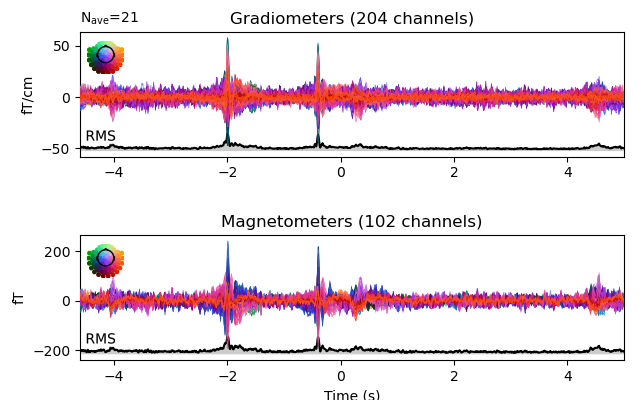
\includegraphics[width=\linewidth]{images_report/sensor/evoked/1_item_short.png}
        \caption{1\_item\_short}
        \label{fig:1_item_short}
    \end{subfigure}\hfil % <-- added
    \begin{subfigure}{0.25\textwidth}
        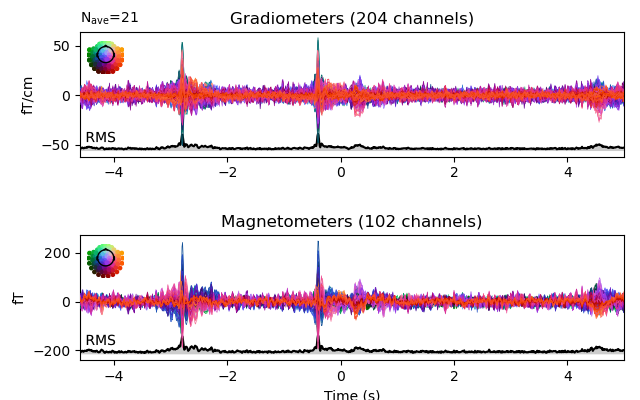
\includegraphics[width=\linewidth]{images_report/sensor/evoked/1_item_medium.png}
        \caption{1\_item\_medium}
        \label{fig:1_item_medium}
    \end{subfigure}\hfil % <-- added
    \begin{subfigure}{0.25\textwidth}
        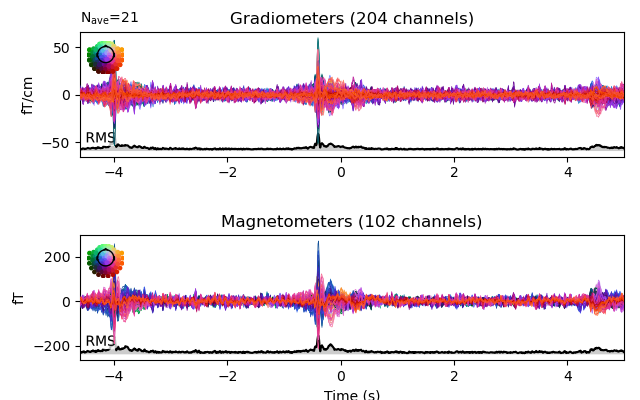
\includegraphics[width=\linewidth]{images_report/sensor/evoked/1_item_long.png}
        \caption{1\_item\_long}
        \label{fig:1_item_long}
    \end{subfigure}

    \medskip
    \begin{subfigure}{0.25\textwidth}
        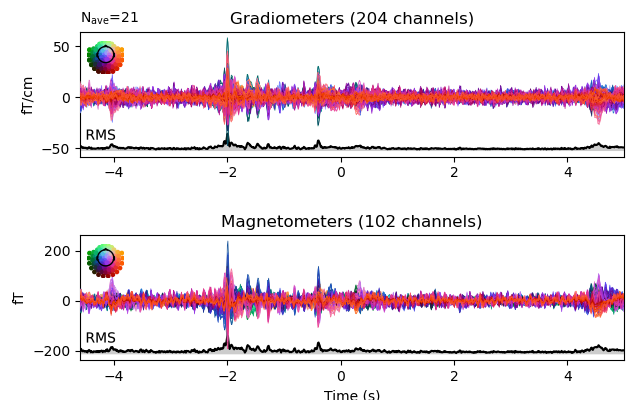
\includegraphics[width=\linewidth]{images_report/sensor/evoked/3_item_short.png}
        \caption{3\_item\_short}
        \label{fig:3_item_short}
    \end{subfigure}\hfil % <-- added
    \begin{subfigure}{0.25\textwidth}
        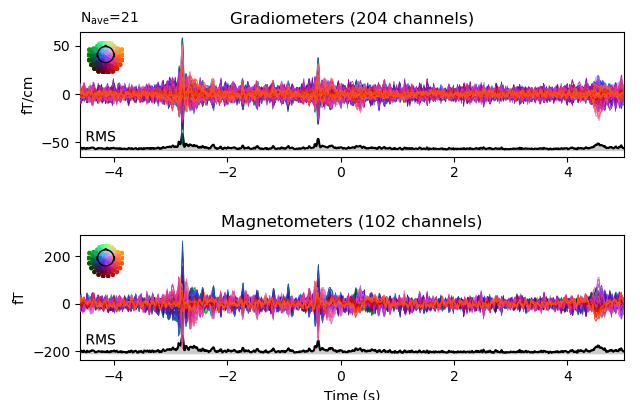
\includegraphics[width=\linewidth]{images_report/sensor/evoked/3_item_medium.png}
        \caption{3\_item\_medium}
        \label{fig:3_item_medium}
    \end{subfigure}\hfil % <-- added
    \begin{subfigure}{0.25\textwidth}
        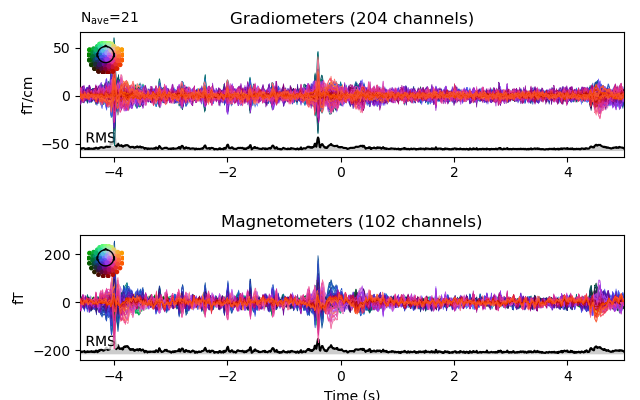
\includegraphics[width=\linewidth]{images_report/sensor/evoked/3_item_long.png}
        \caption{3\_item\_long}
        \label{fig:3_item_long}
    \end{subfigure}
    \caption[Evoked data for our 6 different items.]%
    {Evoked data for our 6 different items.}
    \label{fig:Evoked_data}
\end{figure}


\begin{figure}
    \centering
    \begin{subfigure}{.5\textwidth}
        \centering
        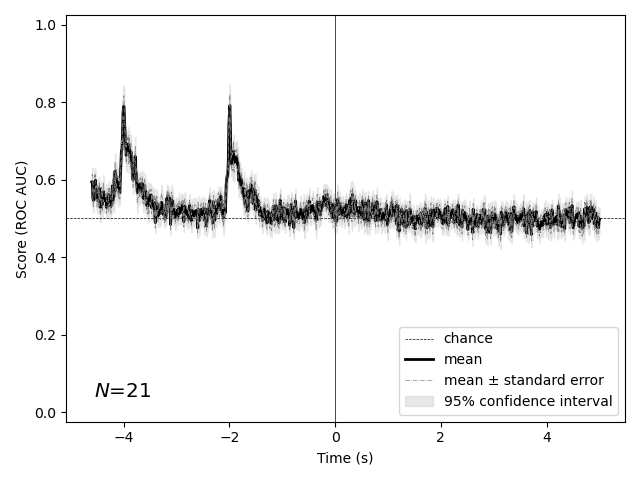
\includegraphics[width=1.\linewidth]{images_report/sensor/contrast/contrast_1_item_short_vs_1_item_long.png}
        \caption{Decoding between 1\_item\_short and 1\_item\_long.}
        \label{fig:decoding_1_item}
    \end{subfigure}%
    \begin{subfigure}{.5\textwidth}
        \centering
        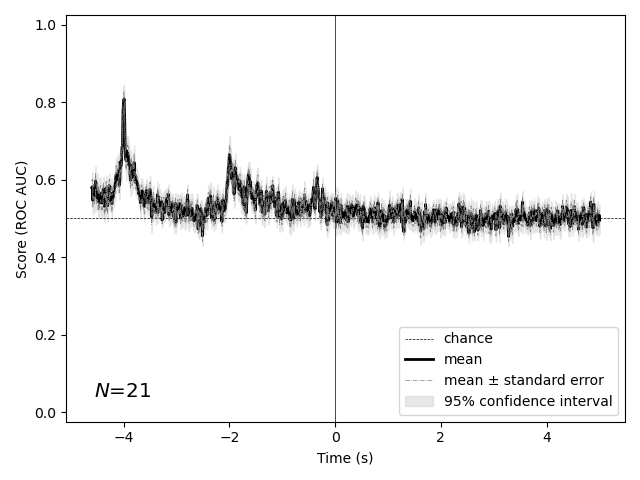
\includegraphics[width=1.\linewidth]{images_report/sensor/contrast/contrast_3_item_short_vs_3_item_long.png}
        \caption{Decoding between 3\_item\_short and 3\_item\_long.}
        \label{fig:decoding_3_item}
    \end{subfigure}
    \caption{Decoding ititialement dans la pipeline.}
    \label{fig:decoding_initial}
    % mettre seulement 1item vs 3 item ici
\end{figure}

\begin{figure}[ht]
    \centering
    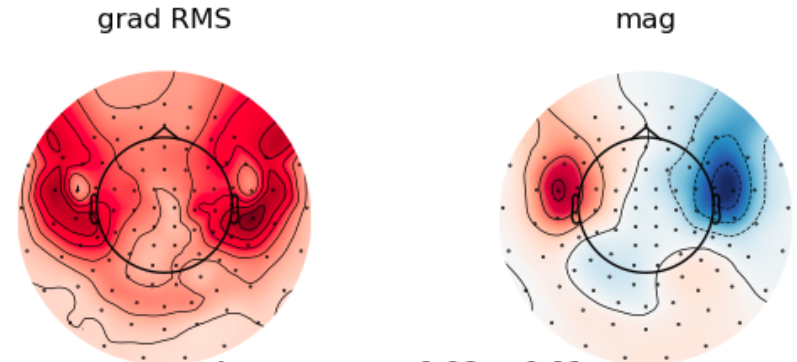
\includegraphics[width=9cm]{images_report/sensor/auditory_cortex.png}
    \caption[Topographic map of the first peak from 1\_item\_short.]%
    {Topographic map of the first peak from 1\_item\_short evoked data \ref{fig:1_item_short}. We can see that during these peaks which appear on the figures \ref{fig:Evoked_data}, it is above all the auditory cortex which is involved.}
    \label{auditory_cortex}
\end{figure}

At the beginning of my internship, the MNE-BIDS-Pipeline allowed us to quickly obtain figures such as \ref{fig:Evoked_data} and such as \ref{fig:decoding_initial}. These figures show that the preprocessing went well since the results are clean. But these two figures also present some limits in the framework of our paradigm:

\begin{itemize}
    \item The figure \ref{fig:Evoked_data} presents the evoked data for each of our 6 different items. The three top figures are temporal sequences containing only one interval (1 item), while the three bottom figures contain sequences of 3 intervals (3 items).
    When there is only one item, we observe two very clear peaks before $t \leq 0$. These two peaks correspond to the pure tone which give the beginning and the end of the interval. After $t \geq 0$ begins the restitution phase, i.e. the phase during which the participant must recall the sequence in his head as precisely as possible. We see that during this restitution phase, the evoked data does not present any particular phenomenon, there is no peak that we could exploit.
    \item In the same way for the figure \ref{fig:decoding_initial}, even if we can see that the decoder used in the pipeline manages to decode the signals before $t=0$ in a very satisfactory way, especially at the location of the auditory stimuli, the performance of the decoders is null during the restitution phase.
\end{itemize}

In this study, we are not interested in the auditory cortex, but in the working memory. We therefore do not concentrate on the listening phase before $t \leq 0$, but rather on the restitution phase after $t \geq 0$. This means that the algorithms that were currently in place in the pipeline were not sufficient at the beginning of my internship, and that we need to find an adequate method to study working memory.

\subsection{Strategy: analysing the contrast in time-frequency space}

Classically the sensor space is decomposed in the following steps:
\begin{itemize}
    \item Computation of the evoked data, by averaging different conditions (i.e. 1 item vs 3 item for us, see figure \ref{fig:Evoked_data} in the results section)
    \item Using a sliding estimator with a logistic regression model for every time point (see figure \ref{fig:decoding_initial} in the results section).
    \item Time frequency decomposition: the epoched data is transformed to time-frequency domain.
    \item Computation of the group average results.
\end{itemize}

This order of operations is fine for most studies. But in the case of our study it is crucial to obtain results in the time-frequency space. We seek here to identify the most salient time-frequencies in order to increase the signal-to-noise ratio when analyzing the contrast in source space. To fill this gap, I implemented a new script in the pipeline to visualize which time-frequency ranges are the most informative with respect to working memory. Concretely, we train a classifier to distinguish the sequences of one item and the sequences of 3 items, and we look at its performance for different frequency ranges, and different time ranges.

We remind you that our working hypothesis is that 3 items load the working memory much more than a single item. The reason for contrasting 3 items with 1 item and not 3 item with 0 item (rest) is that the contrast should not be based on a difference in the nature of the tasks, but rather a difference in load.

My \href{https://github.com/mne-tools/mne-bids-pipeline/pull/414}{pull request} adds a new script to the pipeline, designed to analyze in the time-frequency domain a contrast between two conditions. There are two main steps in this script:
\begin{enumerate}
    \item \textbf{Building the time-frequency map using CSP}: for each time-frequency bin, we use a CSP classifier in order to distinguish between the two conditions. We compute the roc-auc score for each time-frequency bin.
    \item \textbf{Permutation statistics at the group level}: we try to answer the following question: is the difference between the two conditions statistically significant? We use the classic permutations cluster tests on the time-frequency roc-auc map.
\end{enumerate}

\subsection{Building the time-frequency roc-auc map using CSP}

Common Spatial Pattern is based on a geometrical analysis of the brain response, which is called a \textit{pattern}. CSP is used to identify the most salient time-frequencies. We will use CSP to classify between 1-item events and 3-item events. To be able to classify between these two items is to be able to recognize a working memory with two different loads.

We use CSP to identify the most salient times and frequencies for our task: we just have to look at which frequency interval and which time interval our classifier performs best. A good discrimination between the two conditions (1 item vs. 3 items) is characterized by a roc-auc close to 1 while a roc-auc close to 0.5 means that the neural code that encodes the working memory is not detectable by high level geometric features.

\subsection{Decoding with Common Spatial Patterns (CSP)}

CSP is a technique to analyze multichannel data based on recordings from two classes that was introduced in the EEG context by \cite{koles1990spatial}. 

\subsubsection{Intuitive explanation}

% Why CSP better than ...

I took the figure from \cite{blankertz2007optimizing} which also contains a conprehensive tutorial on CSP.

\begin{figure}
    \centering
    \begin{subfigure}{.5\textwidth}
        \centering
        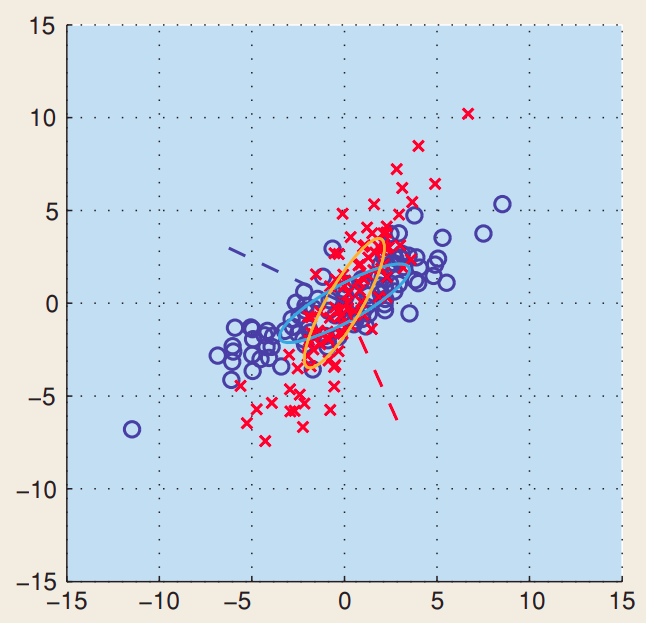
\includegraphics[width=1.\linewidth]{images_report/sensor/before_csp_filtering.png}
        \caption{Before CSP}
        \label{fig:before_csp}
    \end{subfigure}%
    \begin{subfigure}{.5\textwidth}
        \centering
        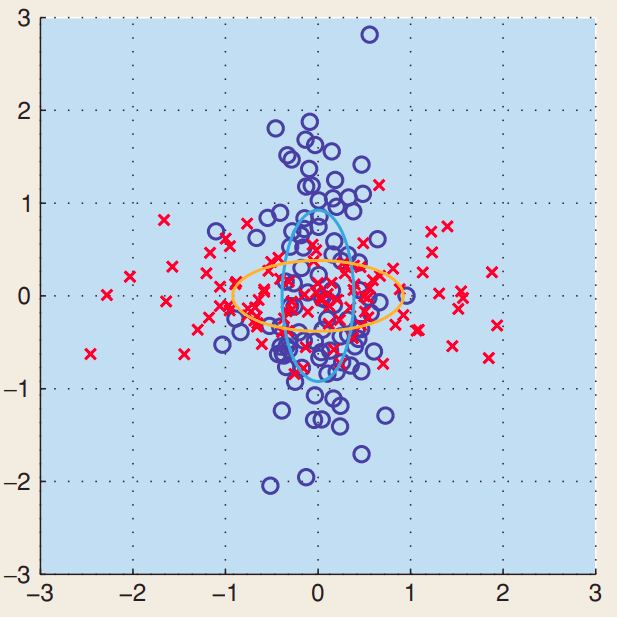
\includegraphics[width=1.\linewidth]{images_report/sensor/after_csp_filtering.png}
        \caption{After CSP transformation}
        \label{fig:after_csp}
    \end{subfigure}
    \caption{Toy example showing the functioning of the CSP transformation.}
    \label{fig:csp_intuitive}
\end{figure}

If we have two Gaussian signals, both centered on the zeros, but with different principal directions, we can try to transform the two point clouds so that the principal directions of the two point clouds in CSP space are orthogonal in order to maximize the ratio of variances along the principal directions.

For example on the figure \ref{fig:csp_intuitive}, we start from two point clouds, red and blue, very correlated, which we transform into decoupled red' and blue' point clouds.

The main vector of the red' cloud is aligned on the x-axis, while the main vector of the blue' cloud is aligned on the y-axis.

By this process, we maximize the variance ratio along the x-axis between the red' and the blue' clouds.

In our usage, a point cloud corresponds to an event, and each color corresponds to a different condition. Here, we do not try to classify points individually as in machine learning, but we classify a whole point cloud. If we try to guess the color/condition of a point cloud, we just have to transform the point cloud with the same transformation as before (i.e. apply the unmixing matrix as we will see later), and take the projection on the x-axis of the new point cloud. We can then calculate the variance along the x-axis and then train a linear classifier to discriminate among the different variances. By combining the CSP algorithm, and for example a logistic regression, we can classify between the two conditions.

\subsubsection{Technical Description (to be skipped in a first reading)}

The above explanation only explains intuitively the algorithm for the first component of the CSP. But it does not explain how to obtain the other orientations. An efficient formulation to obtain all components of the CSP while being computationally reasonable is to formalize the problem as a generalized eigenvector problem.
% [mettre les deux autres formulations]

\paragraph{General Eigenvalue Problem Formulation}

In this section, I use the same notation as in \cite{koles1991quantitative}:

Let $X \in \mathbb{R}^{C \times T}$ be a matrix containing $C$ channels and $T$ time points. The data at a single time point is denoted by $x(t) \in  \mathbb{R}^{C}$. Common spatial pattern (CSP) is a transformation that projects the signal in the original sensor space to CSP space:

\begin{equation}
    x_{\text{CSP}}(t) = W^{T}x(t)
\end{equation}

where each column of $W \in \mathbb{R}^{C  \times C}$ is a spatial filter and each row of $x_{\text{CSP}}(t)$ is a CSP component. Let $\Sigma^{+} \in \mathbb{R}^{C  \times C}$ and $\Sigma^{-} \in \mathbb{R}^{C  \times C}$ be the respective covariance matrices of the two different conditions. CSP analysis is given by the simultaneous diagonalization of the two covariance matrices.


\begin{equation}
    W^{T} \Sigma^{+} W = \lambda^{+}
    \label{eq:lambda_plus}
\end{equation}
\begin{equation}
    W^{T} \Sigma^{-} W = \lambda^{-}
    \label{eq:lambda_minus}
\end{equation}

Where the two $\lambda$ are diagonal matrices whose entries are the eigenvalues of the following generalized eigenvalue problem in $(w, \lambda) \in (\mathbb{R}^{C}, \mathbb{R})$:

\begin{equation}
    \Sigma^{+} w = \lambda \Sigma^{-} w
    \label{eq:general_eigenvalue}
\end{equation}

Large entries in the diagonal matrix corresponds to a spatial filter which gives high variance in one class but low variance in the other. Thus, [en filtrant sur les première componantes] the filter facilitates discrimination between the two classes.

\paragraph{The unmixing matrix}

Another way to read the two equations \ref{eq:lambda_plus} and \ref{eq:lambda_minus} is to remember that $w^{T}\Sigma w$ computes the variance of the covariance $\Sigma$ along the $w$ direction. Thus, $W^{T} \Sigma^{+} W$ and $W^{T} \Sigma^{-} W$ just compute diagonal matrices, whose diagonal elements are the variances of the covariances along the different columns of $W$, namely the variances along the different spatial filters.

By finding all the $w$ which satisfy the equation \ref{eq:general_eigenvalue}, we construct the matrix $W$ also called \textit{unmixing matrix}.

After having found all the couples $(w_i, \lambda_i)$ which satisfy the generalized eigenvalue equation \ref{eq:general_eigenvalue}, we can order the solutions by decreasing eigenvalues. The first filter corresponds to the direction maximizing the ratio of the variances between the two scatter plots. Indeed, if we replace in the equation \ref{eq:lambda_plus}, \ref{eq:lambda_minus}, we obtain:

\begin{equation}
    w^{T}_{i} \Sigma^{+} w_{i} = \lambda^{+}_{i}
    \label{eq:lambda_plus_first_component}
\end{equation}
\begin{equation}
    w^{T}_{i} \Sigma^{-} w_{i} = \lambda^{-}_{i}
    \label{eq:lambda_minus_first_component}
\end{equation}

And it is then enough to replace in \ref{eq:general_eigenvalue} then to multiply on the left by $w^{T}$ to obtain


\begin{equation}
    \lambda_1 = \lambda^{+}_1 / \lambda^{-}_1
\end{equation}

% complement eventuel
% https://www.youtube.com/watch?v=S4znknOIcRk&t=332s
% https://www.youtube.com/watch?v=zsOULC16USU

\subsection{Significance of time-frequency bins with Permutation statistics}

We try to answer the following question: is the difference between
the two conditions statistically significant? We use the a permutations
cluster tests on the time-frequency roc-auc map in order to check the significance of the activation.

\subsubsection{Overview of the cluster permutation statistics method}

\begin{figure}[ht]
    \centering
    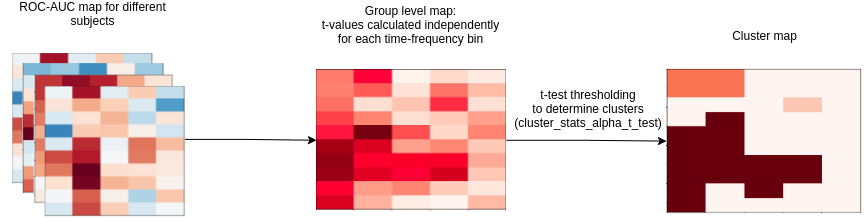
\includegraphics[width=15cm]{images_report/sensor/Permutation_statistics.png}
    \caption[Overview of the permutation statistics pipeline.]%
    {Overview of the permutation statistics pipeline.}
    \label{permutation_statistics_pipeline}
\end{figure}
[harmoniser les images]

The figure \ref{permutation_statistics_pipeline} gives an overview of the cluster creation pipeline.
\begin{enumerate}
    \item We start by collecting all the time-frequency roc-auc maps of all the subjects.
    \item For each time-frequency bin, we compute a t-value, independently for each bin (the details of the computations can be found in the Appendix). We then obtain the t-value map.
    \item Then, in order to find the location of the clusters, we use a threshold, for example corresponding to a chance level of $0.05$ or $0.01$. This threshold is not very important mathematically, but in practice, it allows to control the size of the clusters. Once the threshold is applied, we potentially get one or more clusters.
\end{enumerate}

In order to assign a p-value to each cluster, we have to use the permutation mechanism. The permutation mechanism consists in computing a metric on our clusters: which can be either the size of the cluster, or the maximum of t-values within the cluster, or the sum of t-values within the cluster. [us?] Then we compare this metric to the distribution of this metric simulated for the permutation:
We reverse the sign of the difference for each bin in each subject. We obtain the distribution of the metric in the null hypothesis where the distribution of spatial cluster sizes is independent of the sign of the data.

[detailler]
% going further : threshold free method
% \subsection{Implementation}

\section{Source Space Analysis}

After going into the sensor space. The natural direction is to go to the source space. [ detailler ou retravailler]

\subsection{Generalités source space.}

[Mettre les différents scripts.]

\subsection{New script: Contrast in source space}
Motivation: Insufficient classical pipeline, and inability to average from individual CSPs component.

\begin{figure}[ht]
    \centering
    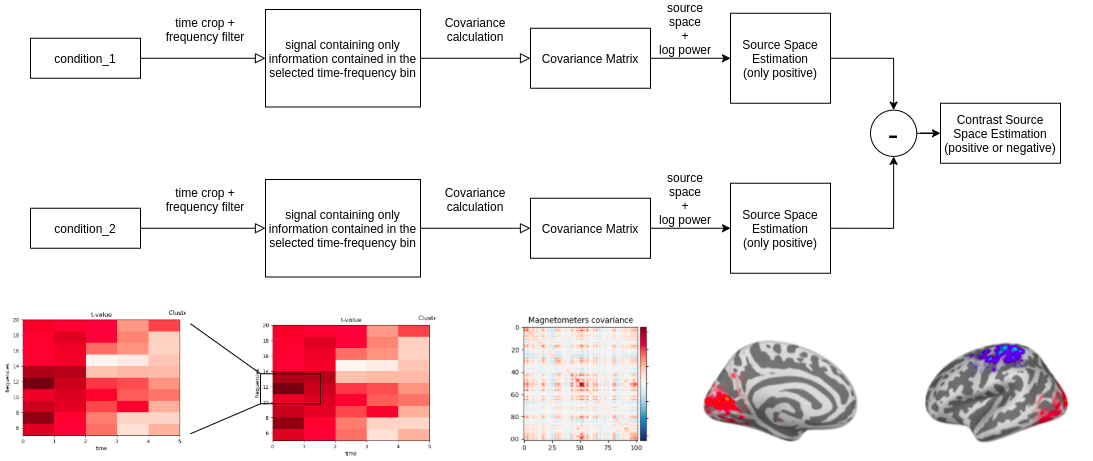
\includegraphics[width=15cm]{images_report/source/flow_source_contrasts.png}
    \caption[Shema of the procedure to visualize the contrast in source space.]%
    {Shema of the procedure to visualize the contrast in source space.}
    \label{flow_source_contrasts}
\end{figure}
